\heading{理论力学-21秋-期中}

\begin{question}[半球碗中的匀质杆]
一个固定的光滑半球形碗，半径为 $R$。一根长为 $L$ 的匀质细杆斜靠在碗边，杆的下端由碗托住，上端伸出碗外。求细杆的平衡位置，并讨论系统存在平衡的条件。用虚功原理求解。

\begin{center}
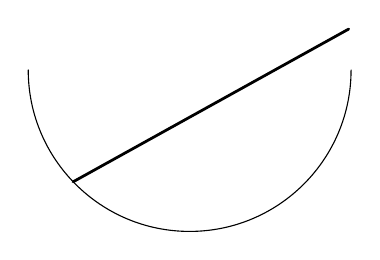
\begin{tikzpicture}[x=1cm,y=1cm,line cap=round,line join=round,font=\small]
  \draw[thin] (-2.05,0) arc[start angle=180,end angle=360,radius=2.05];
  \draw[line width=1pt] (-1.48,-1.42) -- (2.02,0.52);
\end{tikzpicture}

{\small 题 1 示意图}
\end{center}

\begin{solution}
取过杆和碗心的竖直截面。设杆的下端与碗面接触于 $A$，杆经过碗沿点 $B$，碗心为 $O$。令
\[
  \angle AOB=\psi,
  \qquad u=\frac{\psi}{2}.
\]
以 $O$ 为原点、碗沿所在水平线为 $y=0$，取 $B=(R,0)$，则
\[
  A=(R\cos\psi,-R\sin\psi).
\]
于是
\[
  AB=\sqrt{(R-R\cos\psi)^2+(R\sin\psi)^2}=2R\sin u,
\]
且从 $A$ 指向 $B$ 的单位向量为
\[
  \hat{\bm e}_{AB}
  =\frac{B-A}{AB}
  =\bigl(\sin u,\cos u\bigr).
\]
杆的质心 $G$ 距下端 $A$ 的距离为 $L/2$，所以其高度为
\[
  y_G=y_A+\frac L2\cos u
      =-R\sin\psi+\frac L2\cos u
      =\left(\frac L2-2R\sin u\right)\cos u .
\]
所有接触面均光滑，约束力不作虚功，故平衡条件为重力势能 $V=mg y_G$ 对唯一几何变量 $u$ 取驻值：
\[
  \frac{\dd y_G}{\dd u}
  =-\frac L2\sin u-2R\cos 2u=0.
\]
即
\[
  L\sin u+4R\cos 2u=0.
\]
令 $s=\sin u$，利用 $\cos 2u=1-2s^2$，得到
\[
  8Rs^2-Ls-4R=0.
\]
物理上 $0<s<1$，故取正根：
\[
  \boxed{\sin\frac{\psi}{2}
  =\frac{L+\sqrt{L^2+128R^2}}{16R}}.
\]
这就是杆的平衡位置。为了确认它是稳定平衡，可算二阶导数
\[
  \frac{\dd^2y_G}{\dd u^2}
  =-\frac L2\cos u+8R\sin u\cos u
  =\cos u\left(8R\sin u-\frac L2\right).
\]
在上面的平衡根处有 $\sin u>L/(16R)$，且实际根满足 $8R\sin u-L/2>0$，因此对应势能极小。

还需检查几何存在条件。首先平衡根应满足 $s\le 1$：
\[
  \frac{L+\sqrt{L^2+128R^2}}{16R}\le 1
  \quad\Longleftrightarrow\quad L\le 4R.
\]
其次，杆必须至少从下端 $A$ 延伸到碗沿 $B$，即
\[
  L\ge AB=2R\sin u .
\]
代入平衡根，得
\[
  L\ge \frac{L+\sqrt{L^2+128R^2}}8
  \quad\Longleftrightarrow\quad
  7L\ge \sqrt{L^2+128R^2}
  \quad\Longleftrightarrow\quad
  L\ge \sqrt{\frac83}\,R .
\]
故存在这种平衡的条件为
\[
  \boxed{\sqrt{\frac83}\,R\le L\le 4R.}
\]

\end{solution}
\end{question}

\begin{question}[滑块--轻杆系统]
如图，质量为 $M$ 的滑块可沿固定的 $x$ 轴无摩擦滑动，并通过一根长为 $l$ 的轻杆与质量为 $m$ 的质点连接。设轻杆与竖直方向的夹角为 $\theta$。初始条件为 $\theta=0$，$x=0$。

\begin{center}
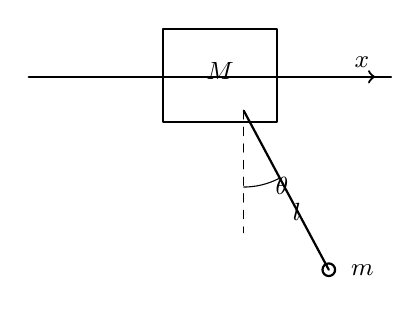
\begin{tikzpicture}[x=1cm,y=1cm,line cap=round,line join=round,font=\small]
  \draw[line width=0.8pt] (-2.25,1.35) -- (2.35,1.35);
  \draw[line width=0.8pt] (-0.55,0.78) rectangle (0.90,1.96);
  \node at (0.18,1.42) {$M$};
  \draw[->,line width=0.8pt] (1.20,1.35) -- (2.15,1.35);
  \node[above] at (1.98,1.35) {$x$};
  \coordinate (P) at (0.48,0.92);
  \coordinate (Q) at (1.56,-1.10);
  \draw[dashed] (P) -- ++(0,-1.55);
  \draw[line width=0.8pt] (P) -- (Q);
  \draw (0.48,-0.05) arc[start angle=-90,end angle=-62,radius=0.97];
  \node[right] at (0.76,-0.03) {$\theta$};
  \node[right] at (0.98,-0.36) {$l$};
  \draw[line width=0.8pt] (Q) circle (0.08);
  \node[right] at (1.72,-1.10) {$m$};
\end{tikzpicture}

{\small 题 2 示意图}
\end{center}

\begin{enumerate}
  \item 写出系统的拉格朗日量，并列出拉格朗日方程，分析系统的运动；
  \item 写出系统的初积分。
\end{enumerate}

\begin{solution}
取滑块坐标 $x$ 与摆角 $\theta$ 为广义坐标。设质点 $m$ 的坐标为 $(X,Y)$，则
\[
  X=x+l\sin\theta,
  \qquad
  Y=-l\cos\theta.
\]
因此
\[
  \dot X=\dot x+l\dot\theta\cos\theta,
  \qquad
  \dot Y=l\dot\theta\sin\theta.
\]
动能为
\begin{align*}
  T&=\frac12M\dot x^2
   +\frac12m(\dot X^2+\dot Y^2) \\
   &=\frac12(M+m)\dot x^2
    +ml\cos\theta\,\dot x\dot\theta
    +\frac12ml^2\dot\theta^2.
\end{align*}
取势能零点任意，令
\[
  V=mgY=-mgl\cos\theta.
\]
故
\[
  L=T-V
  =\frac12(M+m)\dot x^2
    +ml\cos\theta\,\dot x\dot\theta
    +\frac12ml^2\dot\theta^2+mgl\cos\theta .
\]

\begin{enumerate}
  \item 对 $x$ 的拉格朗日方程为
  \[
    \frac{\dd}{\dd t}\frac{\partial L}{\partial \dot x}=0,
  \]
  即
  \[
    (M+m)\ddot x+ml\left(\cos\theta\,\ddot\theta
    -\sin\theta\,\dot\theta^2\right)=0.
  \]
  对 $\theta$ 有
  \[
    \frac{\partial L}{\partial\dot\theta}
    =ml\cos\theta\,\dot x+ml^2\dot\theta,
  \]
  
  \[
    \frac{\partial L}{\partial\theta}
    =-ml\sin\theta\,\dot x\dot\theta-mgl\sin\theta.
  \]
  代入后含 $\sin\theta\dot x\dot\theta$ 的项相消，得到
  \[
    ml\cos\theta\,\ddot x+ml^2\ddot\theta+mgl\sin\theta=0,
  \]
  或
  \[
    \boxed{l\ddot\theta+\cos\theta\,\ddot x+g\sin\theta=0.}
  \]
  两个方程联立给出完整运动。若初始时系统总水平动量为零，则可用动量积分消去 $x$，系统等价为一个具有 $\theta$ 依赖等效惯量的单自由度问题。

  \item 因为 $x$ 是循环坐标，水平总动量守恒：
  \[
    \boxed{p_x=(M+m)\dot x+ml\cos\theta\,\dot\theta=P.}
  \]
  系统不显含时间，因此能量守恒：
  \[
    \boxed{E=\frac12(M+m)\dot x^2
      +ml\cos\theta\,\dot x\dot\theta
      +\frac12ml^2\dot\theta^2-mgl\cos\theta.}
  \]
  若 $P=0$，则
  \[
    \dot x=-\frac{ml\cos\theta}{M+m}\dot\theta.
  \]
  代入能量式得
  \[
    E=\frac12ml^2\frac{M+m\sin^2\theta}{M+m}\dot\theta^2-mgl\cos\theta.
  \]
  于是
  \[
    \dot\theta^2
    =\frac{2(M+m)}{ml^2(M+m\sin^2\theta)}
      \bigl(E+mgl\cos\theta\bigr),
  \]
  它给出 $\theta(t)$ 的一阶积分形式，进而可由 $\dot x$ 求 $x(t)$。
\end{enumerate}
\end{solution}
\end{question}

\begin{question}[圆轨道稳定性]
电子在势场
\[
  U(r)=-\frac{k\ee^{-\alpha r}}{r}
\]
中运动。讨论圆轨道的稳定性。

\begin{solution}
中心力场中角动量 $J=mr^2\dot\varphi$ 守恒，径向运动可写成一维有效势问题：
\[
  E=\frac12m\dot r^2+U_{\mathrm{eff}}(r),
  \qquad
  U_{\mathrm{eff}}(r)=\frac{J^2}{2mr^2}-\frac{k\ee^{-\alpha r}}{r}.
\]
半径为 $a$ 的圆轨道要求 $r=a$ 为有效势驻点：
\[
  U_{\mathrm{eff}}'(a)=0.
\]
直接计算
\[
  U_{\mathrm{eff}}'(r)=-\frac{J^2}{mr^3}
  +k\ee^{-\alpha r}\left(\frac{\alpha}{r}+\frac1{r^2}\right).
\]
所以圆轨道条件为
\[
  \frac{J^2}{m}=ka\ee^{-\alpha a}(1+\alpha a).
\]
稳定性由有效势二阶导数判断。再算
\[
  U_{\mathrm{eff}}''(r)
  =\frac{3J^2}{mr^4}
  -k\ee^{-\alpha r}\left(\frac{\alpha^2}{r}+\frac{2\alpha}{r^2}+\frac2{r^3}\right).
\]
用圆轨道条件消去 $J$，得
\[
  U_{\mathrm{eff}}''(a)
  =\frac{k\ee^{-\alpha a}}{a^3}\bigl(1+\\alpha a-\alpha^2a^2\bigr).
\]
由于 $k\ee^{-\alpha a}/a^3>0$，稳定圆轨道满足
\[
  1+\alpha a-\alpha^2a^2>0.
\]
令 $x=\alpha a>0$，即
\[
  x^2-x-1<0.
\]
因此
\[
  \boxed{0<\alpha a<\frac{1+\sqrt5}{2}.}
\]
当 $\alpha a=(1+\sqrt5)/2$ 时为临界稳定；再大时有效势驻点成为极大，圆轨道不稳定。


\medskip
\textbf{关键步骤：}上述稳定性判据也可由径向小扰动直接得到。令
\[
  r(t)=a+\rho(t),\qquad |
ho|
itimes 0,
\]
角动量 $J$ 保持不变，径向方程在圆轨道附近线性化为
\[
  m\ddot\rho+U_{\mathrm{eff}}''(a)\rho=0.
\]
因此只有当 $U_{\mathrm{eff}}''(a)>0$ 时小扰动才产生振动而不是指数增长；此时径向小振动频率为
\[
  \omega_r^2=\frac{U_{\mathrm{eff}}''(a)}{m}
  =\frac{k\ee^{-\alpha a}}{ma^3}\left(1+\alpha a-\alpha^2a^2\right).
\]
圆轨道条件还说明 $J^2>0$ 自动要求 $1+\alpha a>0$，对 $\alpha>0$ 恒成立；真正限制稳定性的就是二阶导数的符号。


\medskip
本题中 $\alpha^{-1}$ 可理解为相互作用的有效作用程。当 $a$ 很小时，Yukawa 势近似为 Coulomb 势，稳定性条件自然满足；当 $a$ 增大到与作用程同量级以后，吸引力衰减过快，角动量势垒与吸引势的平衡点会变成不稳定点。这一物理图像对应数学条件 $\alpha a<(1+\sqrt5)/2$。
\end{solution}
\end{question}

\begin{question}[去金星的最小发射速度]
将地球与金星绕太阳的轨道都近似看成位于同一平面内的圆轨道，其半径分别为 $R$ 和 $0.7R$。现从地球发射一颗人造卫星前往金星，飞行轨道如图所示。求所需的最小发射速度，并根据题目给定数据计算数值。

\begin{center}
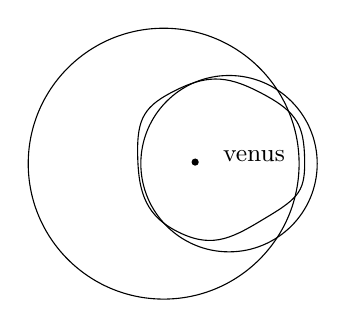
\begin{tikzpicture}[x=1cm,y=1cm,line cap=round,line join=round,font=\small]
  \draw[thin] (-0.45,0) circle (1.72);
  \draw[thin] (0.38,0) circle (1.12);
  \draw[thin] plot[smooth cycle,tension=0.95] coordinates {(1.34,0.07) (0.82,0.88) (-0.28,0.94) (-0.78,0.10) (-0.24,-0.88) (0.86,-0.68)};
  \fill (-0.05,0.02) circle (1.3pt);
  \node[right] at (0.18,0.10) {venus};
\end{tikzpicture}

{\small 题 4 示意图}
\end{center}

\begin{solution}
忽略行星质量对日心转移轨道的影响时，最小能量转移为 Hohmann 转移。设太阳引力参数为
\[
  \mu=GM_\odot,
\]
地球轨道半径为 $r_1=R$，金星轨道半径为 $r_2=0.7R$。转移椭圆的半长轴为
\[
  a_t=\frac{r_1+r_2}{2}=0.85R.
\]
地球绕太阳圆轨道速度为
\[
  v_E=\sqrt{\frac{\mu}{R}}.
\]
转移椭圆在远日点（地球轨道处）的日心速度由 vis-viva 公式给出：
\[
  v_t^2=\mu\left(\frac{2}{r_1}-\frac1{a_t}\right)
  =\frac{\mu}{R}\left(2-\frac{1}{0.85}\right).
\]
因此
\[
  v_t=v_E\sqrt{2-\frac{1}{0.85}}
  \approx 0.9075v_E.
\]
去内侧行星需要降低日心切向速度，故离开地球影响球后的双曲线剩余速度大小为
\[
  v_\infty=v_E-v_t
  =v_E\left(1-\sqrt{2-\frac{1}{0.85}}\right)
  \approx0.0925v_E.
\]
取 $v_E\approx29.8\,\mathrm{km/s}$，得
\[
  v_\infty\approx2.76\,\mathrm{km/s}.
\]
题目要求从地面发射。忽略大气阻力、地球自转和发射纬度影响时，地面处机械能满足
\[
  \frac12v_0^2-\frac{GM_\oplus}{R_\oplus}=\frac12v_\infty^2.
\]
于是
\[
  v_0=\sqrt{v_{\mathrm{esc}}^2+v_\infty^2},
  \qquad
  v_{\mathrm{esc}}=\sqrt{\frac{2GM_\oplus}{R_\oplus}}.
\]
取 $v_{\mathrm{esc}}\approx11.2\,\mathrm{km/s}$，得
\[
  \boxed{v_0\approx\sqrt{(11.2)^2+(2.76)^2}\,\mathrm{km/s}
  \approx11.5\,\mathrm{km/s}.}
\]
方向上，发射后相对于地球的双曲线剩余速度应大致与地球公转速度相反，从而降低卫星的日心能量。


\medskip
\textbf{物理图像：}Hohmann 转移速度来自 vis-viva 公式
\[
  v^2=\mu\left(\frac2r-\frac1a\right).
\]
向内转移时，卫星在地球轨道处的日心速度 $v_t$ 小于地球日心速度 $v_E$，所以发射后的双曲剩余速度方向应与地球公转方向相反。相对地球远离地球后的速度大小为 $v_\infty$；从地面发射还要把地球逃逸能量加进去：
\[
  \frac12v_0^2-\frac{GM_\oplus}{R_\oplus}=\frac12v_\infty^2.
\]
这一区分是本题最容易出错的地方。
\end{solution}
\end{question}

\begin{question}[双匀质杆小振动]
两根均匀细杆位于同一铅垂平面内，质量均为 $m$，长度均为 $l$，并由光滑铰链连接，如图所示。求系统在平衡位置附近作小振动时的频率与运动形式。

\begin{center}
\begin{tikzpicture}[x=1cm,y=1cm,line cap=round,line join=round,font=\small]
  \draw[line width=0.8pt] (-0.95,1.86) -- (0.55,1.86);
  \draw[line width=0.8pt] (0,1.86) -- (0.54,-0.08);
  \draw[line width=0.8pt] (0.54,-0.08) -- (1.32,-1.86);
  \fill (0,1.86) circle (1.3pt);
  \fill (0.54,-0.08) circle (1.3pt);
  \fill (1.32,-1.86) circle (1.3pt);
  \node[left] at (-0.08,1.72) {$O$};
  \node[left] at (0.46,-0.02) {$A$};
  \node[right] at (1.42,-1.84) {$B$};
  \node[right] at (0.30,0.90) {$l$};
  \node[right] at (0.88,-0.96) {$l$};
\end{tikzpicture}

{\small 题 5 示意图}
\end{center}

\begin{solution}
设第一根杆和第二根杆相对竖直向下方向的微小角位移分别为 $\theta_1$、$\theta_2$。两杆的质心坐标为
\[
  \bm r_1=\frac l2(\sin\theta_1,-\cos\theta_1),
\]
\[
  \bm r_2=l(\sin\theta_1,-\cos\theta_1)
  +\frac l2(\sin\theta_2,-\cos\theta_2).
\]
第一根杆绕固定端 $O$ 转动，动能为
\[
  T_1=\frac12\cdot\frac13ml^2\dot\theta_1^2.
\]
第二根杆的质心速度平方为
\[
  v_2^2=l^2\dot\theta_1^2+\frac{l^2}{4}\dot\theta_2^2
  +l^2\dot\theta_1\dot\theta_2\cos(\theta_1-\theta_2),
\]
其绕自身质心转动惯量为 $ml^2/12$，故小振动近似下
\[
  T_2=\frac12m v_2^2+\frac12\frac{ml^2}{12}\dot\theta_2^2
  =\frac12ml^2\dot\theta_1^2
   +\frac12ml^2\dot\theta_1\dot\theta_2
   +\frac16ml^2\dot\theta_2^2.
\]
于是总动能可写为
\[
  T=\frac12ml^2
  \begin{pmatrix}\dot\theta_1&\dot\theta_2\end{pmatrix}
  \begin{pmatrix}
    \frac43&\frac12\\[2pt]
    \frac12&\frac13
  \end{pmatrix}
  \begin{pmatrix}\dot\theta_1\\\dot\theta_2\end{pmatrix}.
\]
势能展开到二阶为
\begin{align*}
  V&=-mg\frac l2\cos\theta_1
    -mg\left(l\cos\theta_1+\frac l2\cos\theta_2\right) \\
   &=\text{常数}+\frac34mgl\theta_1^2+\frac14mgl\theta_2^2+O(\theta^4)  \\
   &=\frac12mgl
  \begin{pmatrix}\theta_1&\theta_2\end{pmatrix}
  \begin{pmatrix}
    \frac32&0\\[2pt]
    0&\frac12
  \end{pmatrix}
  \begin{pmatrix}\theta_1\\\theta_2\end{pmatrix}+\text{常数}.
\end{align*}
因此小振动方程为
\[
  \mathbf M\ddot{\bm\theta}+\mathbf K\bm\theta=0,
\]
其中
\[
  \mathbf M=ml^2
  \begin{pmatrix}
    \frac43&\frac12\\[2pt]
    \frac12&\frac13
  \end{pmatrix},
  \qquad
  \mathbf K=mgl
  \begin{pmatrix}
    \frac32&0\\[2pt]
    0&\frac12
  \end{pmatrix}.
\]
令 $\bm\theta=\bm a\ee^{\ii\omega t}$，并设 $\lambda=\omega^2l/g$，则本征方程为
\[
  \det\left[
  \begin{pmatrix}\frac32&0\\0&\frac12\end{pmatrix}
  -\lambda
  \begin{pmatrix}\frac43&\frac12\\\frac12&\frac13\end{pmatrix}
  \right]=0.
\]
展开得
\[
  \frac34-\frac76\lambda+\frac7{36}\lambda^2=0,
\]
即
\[
  7\lambda^2-42\lambda+27=0.
\]
故
\[
  \lambda_{\pm}=3\pm\frac{6\sqrt7}{7},
  \qquad
  \boxed{\omega_{\pm}=\sqrt{\frac gl\left(3\pm\frac{6\sqrt7}{7}\right)}}.
\]
对应本征矢可由第一行给出
\[
  \left(\frac32-\frac43\lambda\right)a_1-\frac12\lambda a_2=0,
\]
所以
\[
  \frac{a_2}{a_1}=\frac{3}{\lambda}-\frac83.
\]
因此一般小振动解可写为
\[
  \begin{pmatrix}\theta_1\\\theta_2\end{pmatrix}
  =C_+\bm a_+\cos(\omega_+t+\delta_+)
   +C_-\bm a_-\cos(\omega_-t+\delta_-),
\]
其中
\[
  \bm a_\pm=\begin{pmatrix}1\\[2pt]3/\lambda_\pm-8/3\end{pmatrix}.
\]
低频模中两杆大致同向摆动，高频模中两杆反向摆动。
\end{solution}
\end{question}

\begin{question}[圆盘的非完整约束]
在 $x$--$y$ 平面上，一个质量为 $m$、半径为 $R$ 的均匀圆盘作纯滚动。另有约束使盘心到接触点的连线始终垂直于地面平面。
\begin{enumerate}
  \item 分析系统的自由度，并选取合适的广义坐标；
  \item 用拉格朗日乘子法写出系统的运动方程。
\end{enumerate}

\begin{solution}
圆盘始终保持竖直，因此接触点到盘心的连线沿竖直方向。设盘心在水平面上的坐标为 $(x,y)$，圆盘平面在水平面内的方位角为 $\varphi$，圆盘绕自身对称轴滚动的转角为 $\psi$。薄圆盘关于竖直直径方向的转动惯量为
\[
  I_1=\frac14mR^2,
\]
关于自身对称轴的转动惯量为
\[
  I_3=\frac12mR^2.
\]

\begin{enumerate}
  \item 若不考虑无滑动约束，构型变量可取
  \[
    q=(x,y,\varphi,\psi).
  \]
  无滑动滚动给出两个速度约束：
  \[
    \dot x-R\dot\psi\cos\varphi=0,
    \qquad
    \dot y-R\dot\psi\sin\varphi=0.
  \]
  它们将盘心速度限定在圆盘平面方向，且大小等于 $R\dot\psi$。两个约束不是完整约束：例如约束一形式
  \[
    \dd x-R\cos\varphi\,\dd\psi=0,
  \]
  其中系数依赖 $\varphi$，不能全局积分为 $x-R\psi\cos\varphi=\mathrm{const}$。因此该系统是非完整系统。广义坐标数为 $4$，独立速度约束数为 $2$，运动自由度为
  \[
    4-2=2.
  \]

  \item 拉格朗日量为纯动能
  \[
    L=\frac12m(\dot x^2+\dot y^2)
      +\frac12I_1\dot\varphi^2+\frac12I_3\dot\psi^2.
  \]
  用拉格朗日--d'Alembert 乘子法，对约束
  \[
    f_1=\dot x-R\dot\psi\cos\varphi=0,
    \qquad
    f_2=\dot y-R\dot\psi\sin\varphi=0
  \]
  引入乘子 $\lambda_1,\lambda_2$。约束虚功的广义力为
  \[
    Q_i=\lambda_1\frac{\partial f_1}{\partial\dot q_i}
        +\lambda_2\frac{\partial f_2}{\partial\dot q_i}.
  \]
  于是得到
  \[
    m\ddot x=\lambda_1,
    \qquad
    m\ddot y=\lambda_2,
  \]
  \[
    I_1\ddot\varphi=0,
  \]
  \[
    I_3\ddot\psi=-R(\lambda_1\cos\varphi+
    \lambda_2\sin\varphi).
  \]
  再加上两个约束方程
  \[
    \dot x=R\dot\psi\cos\varphi,
    \qquad
    \dot y=R\dot\psi\sin\varphi.
  \]
  这些方程构成非完整系统的运动方程。若进一步消去乘子，可对约束求导：
  \[
    \ddot x=R\ddot\psi\cos\varphi-R\dot\psi\dot\varphi\sin\varphi,
  \]
  \[
    \ddot y=R\ddot\psi\sin\varphi+R\dot\psi\dot\varphi\cos\varphi.
  \]
  从 $\psi$ 方程得到
  \[
    I_3\ddot\psi=-mR(\ddot x\cos\varphi+\ddot y\sin\varphi)
    =-mR^2\ddot\psi.
  \]
  因而
  \[
    (I_3+mR^2)\ddot\psi=0,
    \qquad I_1\ddot\varphi=0.
  \]
  即
  \[
    \dot\psi=\text{常数},
    \qquad
    \dot\varphi=\text{常数}.
  \]
  盘心轨迹由
  \[
    \dot x=R\dot\psi\cos\varphi,
    \qquad
    \dot y=R\dot\psi\sin\varphi
  \]
  给出：若 $\dot\varphi=0$，盘心作直线运动；若 $\dot\varphi\ne0$，盘心作圆周运动。
\end{enumerate}
\end{solution}
\end{question}

\begin{question}[等时摆曲线]
一般单摆的运动周期依赖于振幅。若要求物体在任意振幅下都作简谐运动，问它应沿怎样的曲线运动？请用拉格朗日方法求解。

\begin{solution}
设质点沿某条光滑曲线在竖直平面内无摩擦滑动，用弧长 $s$ 作为广义坐标，并令平衡点为 $s=0$。质点动能为
\[
  T=\frac12m\dot s^2.
\]
若要任意振幅下都作简谐运动，则运动方程必须精确为
\[
  \ddot s+\omega^2s=0,
\]
而不只是小振幅近似。拉格朗日方程给出
\[
  m\ddot s+\frac{\dd V}{\dd s}=0.
\]
因此必须有
\[
  V(s)=\frac12m\omega^2s^2+\text{常数}.
\]
重力势能又为
\[
  V=mgy,
\]
所以曲线高度应满足
\[
  y=\frac{\omega^2}{2g}s^2.
\]
也就是说，若以最低点为原点，曲线上一点的高度正比于从最低点量起的弧长平方。

接下来求满足这一性质的曲线。设曲线用参数 $\theta$ 表为摆线（旋轮线）
\[
  x=a(\theta+\sin\theta),
  \qquad
  y=a(1-\cos\theta),
\]
其中最低点在 $\theta=0$，竖直向上取 $y>0$。其弧长微分为
\[
  \dd s=\sqrt{(\dd x)^2+(\dd y)^2}
  =a\sqrt{(1+\cos\theta)^2+\sin^2\theta}\,\dd\theta
  =2a\cos\frac\theta2\,\dd\theta.
\]
故
\[
  s=\int_0^\theta 2a\cos\frac{\theta'}2\,\dd\theta'
   =4a\sin\frac\theta2.
\]
同时
\[
  y=a(1-\cos\theta)=2a\sin^2\frac\theta2
  =\frac{s^2}{8a}.
\]
于是
\[
  V=mgy=\frac{mg}{8a}s^2.
\]
与 $V=\frac12m\omega^2s^2$ 比较得
\[
  \omega^2=\frac{g}{4a}.
\]
因此运动方程为
\[
  \ddot s+\frac{g}{4a}s=0,
\]
周期为
\[
  T=2\pi\sqrt{\frac{4a}{g}},
\]
与振幅无关。所求曲线为
\[
  \boxed{x=a(\theta+\sin\theta),
  \qquad y=a(1-\cos\theta),}
\]
即摆线。根据取向不同，也可写成等价形式 $x=a(\theta-\sin\theta)$、$y=a(1-\cos\theta)$。


\medskip
\textbf{几何核查：}对摆线参数式
\[
  x=a(\theta+\sin\theta),\qquad y=a(1-\cos\theta),
\]
有
\[
  \frac{\dd x}{\dd\theta}=a(1+\cos\theta),
  \qquad
  \frac{\dd y}{\dd\theta}=a\sin\theta.
\]
故弧长微元为
\[
  \dd s=a\sqrt{(1+\cos\theta)^2+\sin^2\theta}\,\dd\theta
  =2a\cos\frac\theta2\,\dd\theta,
\]
从最低点起积分得到 $s=4a\sin(\theta/2)$。代回高度 $y=2a\sin^2(\theta/2)$，确有 $y=s^2/(8a)$，因此运动方程严格线性，而不是小振幅近似线性。
\end{solution}
\end{question}

\begin{question}[卢瑟福散射]
考虑势能
\[
  V(r)=\frac{k}{r}
\]
下的散射问题。设入射粒子的能量为 $E$，推导卢瑟福散射公式。

\begin{solution}
设入射粒子在无穷远处的速度为 $v$，则
\[
  E=\frac12mv^2.
\]
碰撞参数为 $b$，角动量为
\[
  J=mvb.
\]
中心力散射中轨道方程可由 Binet 方程得到。令 $u=1/r$，对斥力势 $V=k/r$，有
\[
  F(r)=-\frac{\dd V}{\dd r}=\frac{k}{r^2}.
\]
Binet 方程为
\[
  \frac{\dd^2u}{\dd\varphi^2}+u=-\frac{mF(1/u)}{J^2u^2}
  =-\frac{mk}{J^2}.
\]
其解为
\[
  u=A\cos(\varphi-\varphi_0)-\frac{mk}{J^2}.
\]
这是一条双曲线。由能量关系可得偏心率
\[
  e=\sqrt{1+\frac{2EJ^2}{mk^2}}.
\]
将 $J=mvb$ 与 $E=mv^2/2$ 代入，得
\[
  e=\sqrt{1+\frac{4E^2b^2}{k^2}}.
\]
双曲线两条渐近线之间的偏转角 $\chi$ 满足
\[
  \tan\frac\chi2=\frac{1}{\sqrt{e^2-1}}.
\]
于是
\[
  \tan\frac\chi2=\frac{k}{2Eb},
  \qquad
  \boxed{b=\frac{k}{2E}\cot\frac\chi2.}
\]
散射截面的定义为：落在 $b$ 到 $b+\dd b$ 环带中的粒子，散射到立体角 $\dd\Omega=2\pi\sin\chi\,\dd\chi$ 中。故
\[
  \dd\sigma=2\pi b\,|\dd b|,
\]
从而
\[
  \frac{\dd\sigma}{\dd\Omega}
  =\frac{b}{\sin\chi}\left|\frac{\dd b}{\dd\chi}\right|.
\]
由
\[
  b=\frac{k}{2E}\cot\frac\chi2
\]
可得
\[
  \left|\frac{\dd b}{\dd\chi}\right|
  =\frac{k}{4E}\csc^2\frac\chi2.
\]
再用
\[
  \sin\chi=2\sin\frac\chi2\cos\frac\chi2,
  \qquad
  \cot\frac\chi2=\frac{\cos(\chi/2)}{\sin(\chi/2)},
\]
得到
\begin{align*}
  \frac{\dd\sigma}{\dd\Omega}
  &=\frac{1}{2\sin(\chi/2)\cos(\chi/2)}
    \left(\frac{k}{2E}\frac{\cos(\chi/2)}{\sin(\chi/2)}\right)
    \left(\frac{k}{4E}\csc^2\frac\chi2\right) \\
  &=\frac{k^2}{16E^2}\csc^4\frac\chi2.
\end{align*}
因此卢瑟福散射公式为
\[
  \boxed{\frac{\dd\sigma}{\dd\Omega}
  =\frac{k^2}{16E^2\sin^4(\chi/2)}.}
\]
若 $k=q_1q_2/(4\pi\varepsilon_0)$，代入即可得到电荷散射的通常形式。该结果对库仑斥力成立；吸引情形只改变轨道几何取向，截面公式形式相同。
\end{solution}
\end{question}
